\documentclass[border=12pt]{standalone}
\usepackage{tikz}
\usetikzlibrary{positioning, calc, arrows.meta, fit, backgrounds}

\definecolor{fusion}{HTML}{C7B8FF}
\definecolor{trunk}{HTML}{B4D4FF}

\begin{document}

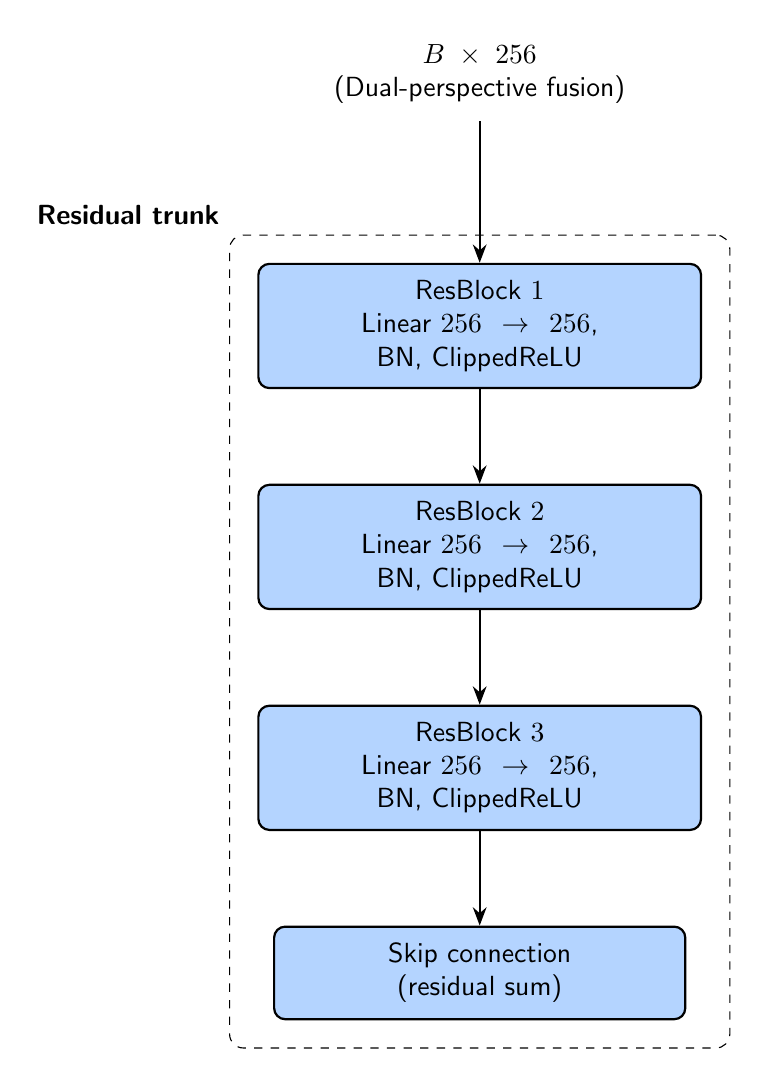
\begin{tikzpicture}[
    >=Stealth,
    thick,
    font=\sffamily,
    node distance=1.4cm and 1.6cm,
    block/.style={
        draw,
        rounded corners=4pt,
        align=center,
        minimum height=1.0cm,
        text width=5.2cm,
        inner sep=6pt
    },
    trunk/.style={block, fill=trunk},
    merge/.style={block, fill=none, draw=none},
    groupbox/.style={
        draw,
        rounded corners=5pt,
        dashed,
        inner sep=10pt,
        label={[font=\bfseries\sffamily]north west:#1}
    }
]

\node[merge] (H) {$B \times 256$\\ (Dual-perspective fusion)};
\node[trunk, below=1.8cm of H] (R1) {ResBlock $1$\\Linear $256\to256$, BN, ClippedReLU};
\node[trunk, below=1.2cm of R1] (R2) {ResBlock $2$\\Linear $256\to256$, BN, ClippedReLU};
\node[trunk, below=1.2cm of R2] (R3) {ResBlock $3$\\Linear $256\to256$, BN, ClippedReLU};
\node[trunk, below=1.2cm of R3, text width=4.8cm] (Skip) {Skip connection\\(residual sum)};

\draw[->] (H) -- (R1);
\draw[->] (R1) -- (R2);
\draw[->] (R2) -- (R3);
\draw[->] (R3) -- (Skip);

\begin{scope}[on background layer]
  \node[groupbox=Residual trunk, fit=(R1)(R2)(R3)(Skip)] {};
\end{scope}

\end{tikzpicture}

\end{document}
